% Standalone render of the four-layer constraint architecture figure.
% Same TikZ source as the paper's fig:constraint-architecture.
\documentclass[tikz,border=6pt]{standalone}
\usepackage{tikz}
\usetikzlibrary{positioning}
\begin{document}
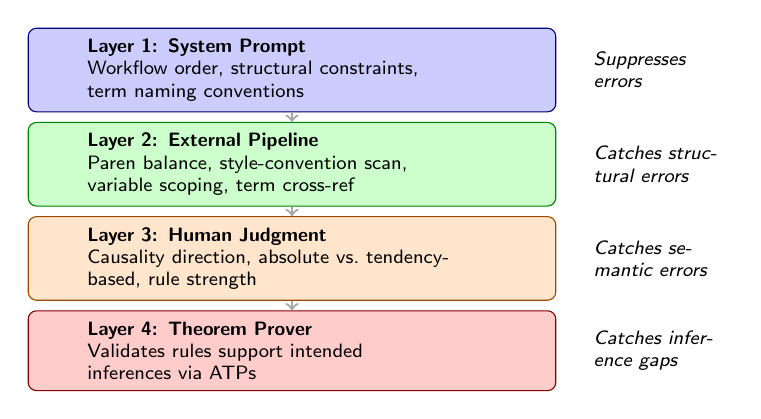
\begin{tikzpicture}[
    node distance=0.12cm,
    layer/.style={
        rectangle, rounded corners=3pt,
        minimum width=6.7cm, minimum height=0.6cm,
        text width=5.2cm, align=left,
        font=\scriptsize\sffamily, inner sep=4pt
    },
    label/.style={
        font=\scriptsize\sffamily\itshape,
        text width=1.65cm, align=left
    }
]

%% Layer boxes (top to bottom)
\node[layer, fill=blue!20, draw=blue!50!black]
    (L1) {\textbf{Layer 1: System Prompt}\\
          Workflow order, structural constraints,\\
          term naming conventions};

\node[layer, fill=green!20, draw=green!50!black, below=of L1]
    (L2) {\textbf{Layer 2: External Pipeline}\\
          Paren balance, style-convention scan,\\
          variable scoping, term cross-ref};

\node[layer, fill=orange!20, draw=orange!60!black, below=of L2]
    (L3) {\textbf{Layer 3: Human Judgment}\\
          Causality direction, absolute vs.\
          tendency-based, rule strength};

\node[layer, fill=red!20, draw=red!50!black, below=of L3]
    (L4) {\textbf{Layer 4: Theorem Prover}\\
          Validates rules support intended\\
          inferences via ATPs};

%% Right-side labels
\node[label, right=0.35cm of L1] {Suppresses errors};
\node[label, right=0.35cm of L2] {Catches structural errors};
\node[label, right=0.35cm of L3] {Catches semantic errors};
\node[label, right=0.35cm of L4] {Catches inference gaps};

%% Arrows between layers
\draw[->, thick, gray!70] (L1.south) -- (L2.north);
\draw[->, thick, gray!70] (L2.south) -- (L3.north);
\draw[->, thick, gray!70] (L3.south) -- (L4.north);

\end{tikzpicture}
\end{document}
